\documentclass{article}
\usepackage{draftwatermark}
\usepackage{longtable}
\SetWatermarkText{DRAFT}
\SetWatermarkScale{1}

\author{Michael Edwards\\ 
  James Woods}
\title{Housing Market Institutions Drive Race and Ethnicity Differences in Energy Consumption}


\usepackage{Sweave}
\begin{document}
\maketitle
\Sconcordance{concordance:DraftEdwardsWoods.tex:DraftEdwardsWoods.Rnw:%
1 10 1 1 0 12 1 1 310 1 7 6 1 1 3 16 0 1 2 4 1 1 3 1 2 8 1 1 3 1 2 13 1 %
1 8 62 0 1 3 4 1 1 15 100 0 1 2 2 1 1 7 46 0 1 3 1 1 1 6 16 0 1 1 223 0 %
1 3 4 1 1 50 10 1}


\begin{abstract}

When socio-demographic factors are considered in any kind of analysis of household electric and gas utility data, it is common to observe differences in energy use between households with different self-reported race and ethnicity compositions. These differences persist controlling for structure type, e.g., single family dwelling, age and size of housing units, and, other common control variables. Without the information necessary to better explain these differences, they are commonly summarized simply as cultural differences. This paper demonstrates that these differences can be partially explained by differential sorting by structure and ownership, i.e., endogenizing housing choice and rental decisions. We will show that these differences in energy consumption may be because of housing market institutions and restrictions.
\end{abstract}

\section{Introduction}

The choice of housing, differentiated between renters and owners: owners and those households making payments towards ownership are treated as the same.  Homes are categorized by structure type.   

Housing choices may be linked to fundamental characteristics of the heads of households as a dependent variable that has implications as to utility, and in this respect it is assumed that owning a detached home is of greatest use.  The choice of homes is considered cardinal, where a house is of greatest value and the mobile home is treated as the least appealing choice.  A townhome, row house, in a desirable location such as an urban area, may be a highly desirable good, in general that is not treated as the norm. Structures other than detached houses may be considerably more perishable.  This assumption is made regardless of variations within the desirability of particular detached houses. The choice of purchasing or renting a home is relevant within the structure types.  An individual may choose to forego ownership of a townhouse in favor of renting a house, or forego owning a mobile home in favor of renting an apartment.  Here, both from a utilitarian perspective of the need for one domicile over another is considered as well as prestige that comes from both the structure type as well as what utility may derive from ownership.

The value of structure type may have implications as to future wealth.  Homeowners tend towards greater wealth over time, related to home ownership itself(Di 2007).  Homeowners have the opportunity to use their wealth for investment or paying off higher interest debts, such as credit cards, by using home equity.  Homeowners have access to a safety net in terms of debt, and they also have the opportunity of reducing the lifetime costs of debts.  Homeowners may also choose to liquidate their homes, or pass on wealth at at or near the end of their lives.  One source found homeowners held more wealth compared to their contemporary counterparts.  The growth of wealth was also appreciably higher(Di 2007). 
  
The effect of home ownership and structure choice may have implications for future outcomes of the children of the suggested households.  In that respect, it can be said that there is evidence of children having better outcomes, in terms of education and income, than their peers in households that choose to rent (Boehm 2014).  It is plausible that the outcome benefits are coming from a causal relationship with parental characteristics rather than that of the housing choice, and are co-variables, rather than having an internal causal relationship.  While it is beyond the scope of this paper, it is also plausible that housing choice is indicative of neighborhood choice, though it should be stated that there is no assertion on this statement to be found here.

Households choice of structure type, payment method, and location are often very difficult to change based on the history of a household (Darrah 2014).  Households that have tended towards renting have difficulty, or at least choose not to, buy in the future.  Community attitudes and behaviors in relation to housing are often sticky in changing, and this is of importance as related to the outcomes of children; often mirroring the characteristics of their parents.  


This paper explores the relationship between the household characteristics and the choice of housing structure, and suggests that there is reason in particular of choosing housing structures based on wealth and needs as a proxy for utility, which not only has immediate effects but those that have persistent effects on the legacy of households.  While the utility of a particular domicile cannot be measured directly, it is assumed that the choice of structure is indicative of the value that the household places on one choice over another.  


% \begin{itemize}
% 
%   \item Differences in energy use by race and ethnicity is frequently reported in the literature
%   \item Much of the difference has to do with differences in income levels and education but not frequently modeled correctly.
%   \item Even with proper race and ethnicity controls with income, some patterns persist.
%   \item We assert that these differences are caused, at least in part, by housing discrimination, forcing people into housing types different than what they would prefer without discrimination; and renting rather than buying.
%   \item We show this with a model that endogenizes structure type and tenure decision.
%   \item emphasize that this is early work.
% \end{itemize}

%\cite{RBase}




  \subsection{Race and Ethnicity in Conditional Demand}
  
  \subsection{How Race and Ethnicity are Interpreted}

\section{RECS}

The 2009 Residential Energy Consumption Survey (RECS) was the main source of data. 12083 observations are included in the data, of which 11905 are used for most of the models. Because of the complex sampling scheme, which involves both cluster sampling and over sampling of odd cells, weights are used in all analysis.  The reason that the majority of the observations were dropped was because the households were living on premises for free, neither owning or renting the property.  We also dropped a few observations because they were under-sampled and the post-stratification weights  were so large to as not be credible.


The RECS data set contains information on both the dwelling structure type,  and an indicator if they own the property.  The dwelling types are divided into the six common categories: single family detached house, single family attached (including duplexes and row house, small apartment complexes, large apartment complexes, and mobile homes. 

The RECS survey contains an enormous number of variables, 931, for each household including: income, resident ages, education, rental assistance, appliance and building characteristics, thermostat set-points, householder ethnicity and race.  Income was recorded in categories but midpoints of the categories were used for most analysis. 
% 
% Over twice as many households choose to own their homes compared to renters.  As well we see that the majority of households, more than all other categories combined, live in single family detached houses (See Appendix).  Behind single family houses, large apartment complexes were the most likely dwelling types chosen.  Notably, apartments in general, were more commonly rented than owned as compared to the opposite for each other dwelling type.
% 
% With respect to respondent education attainment, percentages of each category (see appendix) do differ from what can be expected.  It is entirely likely that this is an example of the survey effect on selection of respondents, i.e. that individuals with higher education attainment are more likely to respond to mailed surveys.   	


% RECS data set is the 2009 publication.  12083 observations are included in the data, of which 11395 are included in the struture-tenure model. Combining dwelling type (dwltype) and the binary response variable Ownrent, Dwltype includes six categories as follows: single family detached house, townhouse (including duplex, or row house), small apartment complex, large apartment complex, mobile home. Mobile homes are notable for having considerably fewer observations than other categories. The model is based on the following variables: income, resident ages, education, and ethnicity.  Logged, midpoints, are used for income. Education is broken into six categories describing highest education level completed by the head of the household: elementary, some high school, high school. Some college/trade/vocational school, college graduate and post graduate degree.  The ethnicity variable is constructed from a composite of six dummy variables for head of households broken into head of households one and two.  The result is one variable for each where from one to six: Native American, Asian/Pacific Islander, Black/African American, Hispanic/Latino, White/Caucasian, and Other.  For our purposes head of household \#2 is ignored.

% 	Approximately 2.7 times as many households choose to own their homes compared to renters.  As well we see that the majority of households, more than all other categories combined, live in singe family detached houses (See Appendix).  Behind single family houses, large apartment complexes were the most likely dwelling types chosen.  Notably, apartments in general, were more commonly rented than owned as compared to the opposite for each other dwelling type.
  
% 	With respect to respondent education attainment, it can be noted that the percentages of each category (see appendix) do differ from that of what can be expected.  It is entirely likely that this is an example of the survey effect on selection of respondents, i.e. that individuals with higher education attainment are more likely to respond to mailed surveys.  Comparing to a cursory internet search for example, more respondents hold graduate degrees and bachelor’s degrees, and less high school diplomas and below than that percentage constructed for the state of California (PPIC).  It is also of minor interest to note the seventy-nine respondents who claim to live in mobile homes and hold graduate degrees.  While that combination of characteristics is plausible enough without further examination, it does bring into question the honesty of respondent’s self-reported information.  But, by constructing a variable equal to the number of housemates over the age of 65 and tabulating it against just mobile homes within the dwelling type variable, we note that the majority of respondents state that 1346 seniors live in mobile homes compared to 643 mobile homes without senior citizens, which is a considerably different trend than homes largely without seniors in the other dwelling type categories particularly detached houses, bearing in mind that this is relatively and the majority of seniors recorded in the data do not live in mobile homes. This may suggests that seniors are utilizing mobile homes as retirement homes, possibly within retirement communities and that would help to explain the minor perceived discrepancy in the education variable.  It is also commonly held that seniors may be more likely to respond to surveys, much like voting, and this would suggest why there are more respondents in mobile homes than in every other category of dwelling aside from home ownership and small complex ownership.  It can be noted from the RASS survey that, in fact, mobile homes had the highest response rate (RASS).
% 	
% Lastly, one of our variables, actually two, are count variables that account for the number of children under the age of five and between six and eighteen respectively.  This variable was constructed with the intention of finding whether larger structures, in general, such as houses and townhouses, are chosen more often by individuals requiring more room or who are exhibiting more permanent nesting behavior, as in choosing to purchase a home with the intention of residing there for a long period of time and becoming well established.



% Adding in some basic descriptors

Table 
 \ref{tab:RaceVStruct}
shows the count of observations by Race/Ethnicity and structure after the basic data handling described above.  Please note the dominance of single family detached homes, shown as SFDetached in the table and non-Hispanic Caucasians, shown as FALSEWt in the table.  These counts are unweighted and do not take into account the stratified sampling scheme used to collect the data.

% latex table generated in R 3.0.1 by xtable 1.7-4 package
% Tue Apr  7 18:17:42 2015
\begin{table}[ht]
\centering
\caption{Count of Observations by Race and Structure Type} 
\label{tab:RaceVStruct}
{\small
\begin{tabular}{rrrrrr}
  \hline
 & Mobile & SFDetached & SFAttached & SmApartment & LgApartment \\ 
  \hline
FALSEWt & 371 & 5694 & 544 & 430 & 951 \\ 
  FALSEAfAm &  24 & 754 & 121 & 174 & 382 \\ 
  FALSEAsian &   1 & 231 &  48 &  52 & 113 \\ 
  FALSEMulti &   6 &  87 &  14 &  12 &  27 \\ 
  FALSENativeAm &   7 &  35 &   9 &   7 &  15 \\ 
  FALSEOther &   2 &  59 &   8 &  13 &  29 \\ 
  FALSEPacific &   1 &  22 &   1 &   2 &  10 \\ 
  TRUEAfAm &   3 &   8 &  10 &   5 &   8 \\ 
  TRUEAsian &   0 &   5 &   0 &   0 &   1 \\ 
  TRUEMulti &   1 &  10 &   2 &   4 &   4 \\ 
  TRUENativeAm &   2 &  17 &   3 &   6 &   9 \\ 
  TRUEOther &   6 &  41 &  12 &  16 &  24 \\ 
  TRUEPacific &   0 &   2 &   1 &   1 &   0 \\ 
  TRUEWt &  97 & 730 & 105 & 184 & 332 \\ 
   \hline
\end{tabular}
}
\end{table}
Many of the structure type/ race and ethnicity combinations are relatively rare, e.g., Hispanic Asians living in mobile homes.  We have not collapsed any of these  categories.  Future research will look at collapsing some of the rare cells so that there are a more manageable number of both structure types and race/ethnicity combinations.


Table
\ref{tab:RegionVStruct}
gives a further description of the data is distributed around the country.  Please note that both the Western and North Eastern area have a larger fraction of large apartment buildings, LgApartment in the table, than the other two regions. 


% latex table generated in R 3.0.1 by xtable 1.7-4 package
% Tue Apr  7 18:17:42 2015
\begin{table}[ht]
\centering
\caption{Count of Observations by Region and Structure Type} 
\label{tab:RegionVStruct}
{\small
\begin{tabular}{rrrrr}
  \hline
 & NE & MidWest & South & West \\ 
  \hline
Mobile &  47 &  92 & 245 & 137 \\ 
  SFDetached & 1173 & 2080 & 2685 & 1757 \\ 
  SFAttached & 218 & 162 & 257 & 241 \\ 
  SmApartment & 326 & 145 & 226 & 209 \\ 
  LgApartment & 470 & 323 & 603 & 509 \\ 
   \hline
\end{tabular}
}
\end{table}
The table shows the range of climate zones and housing law covered by the survey.  It also shows the reasonableness of our hypotheses that location and structure type choices are endogenous.

Figure
\ref{fig:kWhbyOwnRace}
shows a smooth approximation of the distribution of annual household electricity use in kWh per year.  The columns indicates the various self-identified race and the columns indicate if the the household self identifies as Hispanic and if the home is owned or rented. The blank cells indicate that there are too few observations to generate a reliable smooth approximation of electricity consumption.

Please note that households that rent tend to have lower annual electricity consumption and a smaller variance in that consumption.  This is normal given that rented apartments which are typically smaller and of more uniform size than single family dwellings.  

\begin{figure}[htbp]
\begin{center}
\caption{Annual kWh by Rent/Own and Race}
\label{fig:kWhbyOwnRace}
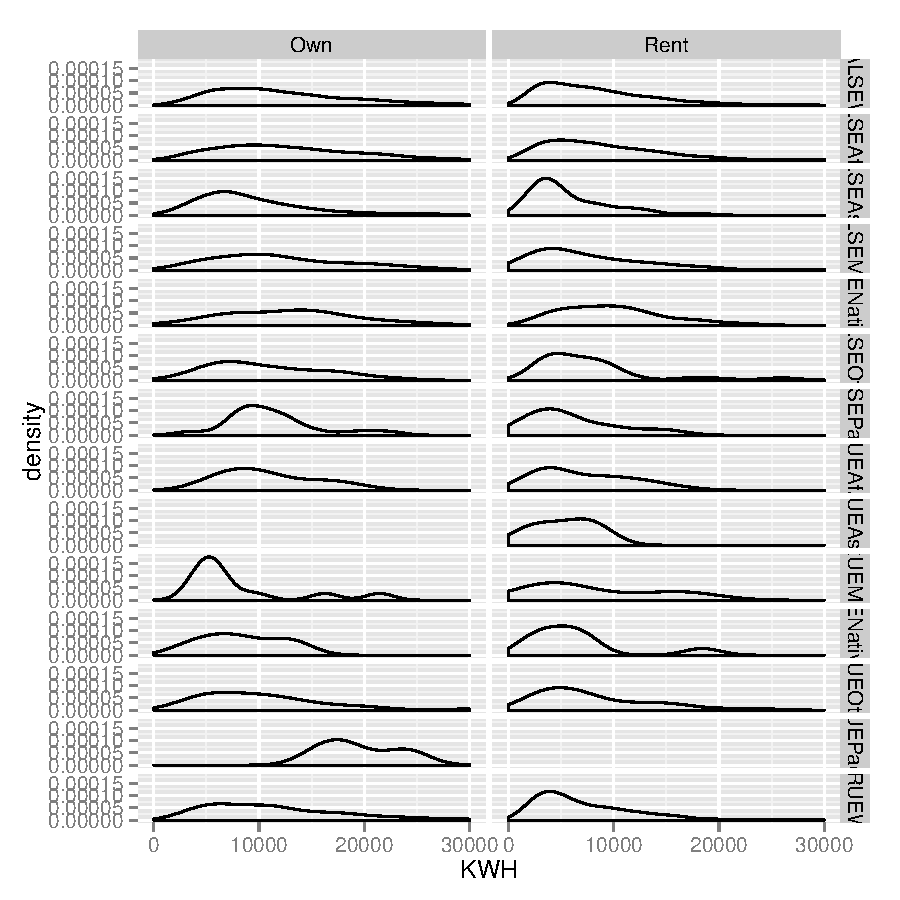
\includegraphics{DraftEdwardsWoods-005}
\end{center}
\end{figure}


  \subsection{Race and Ethnicity Differences in Equipment and Structure}

There are many choices that are frequently thought of as exogenous in conditional demand models that could account for differences electricity consumption by race and ethnicity.  One of the most obvious is the location of the residence.  At the most basic level, choosing to locate a household drives energy consumption.  

Figure 
\ref{fig:UrbanRural}
shows the one of the most basic locational choices, residing in an urban or rural area.  Race is represented by the columns and the two rows, labeled FALSE and TRUE, indicate if the household self identifies as Hispanic, TRUE, or not.  The bars represent the fraction of each race and ethnicity combination that reside in rural and urban areas.

\begin{figure}[htbp]
\begin{center}
\caption{Urban vs Rural by Race and Ethnicity}
\label{fig:UrbanRural}
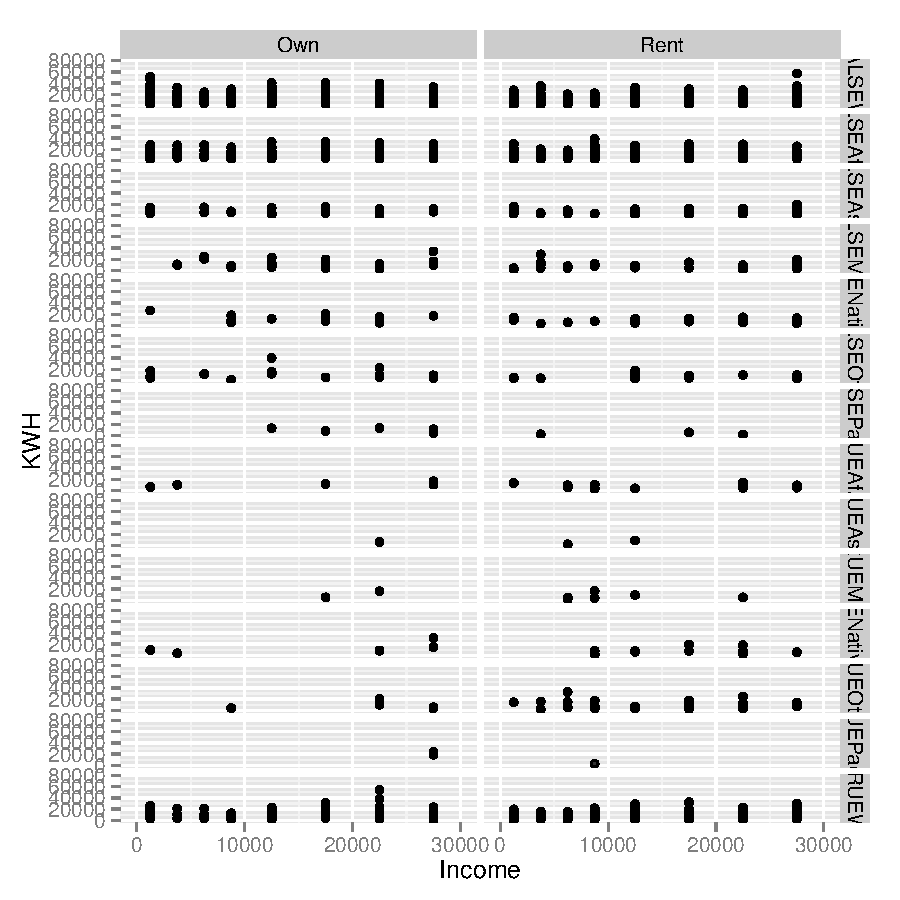
\includegraphics{DraftEdwardsWoods-006}
\end{center}
\end{figure}

Non-Hispanic Caucasian and Native American households are more likely to reside in a rural area while those that identify as Hispanic are, in each category, almost always more likely to live in urban areas than those that don't self-identify as Hispanic.  The connection to energy consumption is through the correlation between rural households having larger residences that are more likely to be single family detached houses. 

Some of the large differences in those self-identified Hispanic categories are because of very sparse cells.  There are only four Hispanic Pacific Islanders in the survey.

Both the water and space heating fuel show significant differences across race and ethnicity combinations.  The fuel choice something controlled by the owner of the structure.  For households that rent this choice more likely to be electric heating and water service.  While electric heat and water service is often very expensive on a month-to-month basis, the installation costs are typically quite low.  The installation cost is what is faced by the landlord.  The month-to-month cost is faced by the lessee.

Figure \ref{fig:HeatFuel} shows the distribution of heating fuel by race and ethnicity.  It is very clear that Natural Gas is the most common fuel for hot water service but there are some differences based on race and ethnicity.  Excluding the less common self-identified Hispanic categories, native Americans and pacific islanders are more likely to have electric hot water service than non-Hispanic Caucasians and households with a head of household that identifies as multi-racial is less likely to have electric hot water service.  

\begin{figure}[htbp]
\begin{center}
\caption{Water Service by Race and Ethnicity}
\label{fig:WaterService}
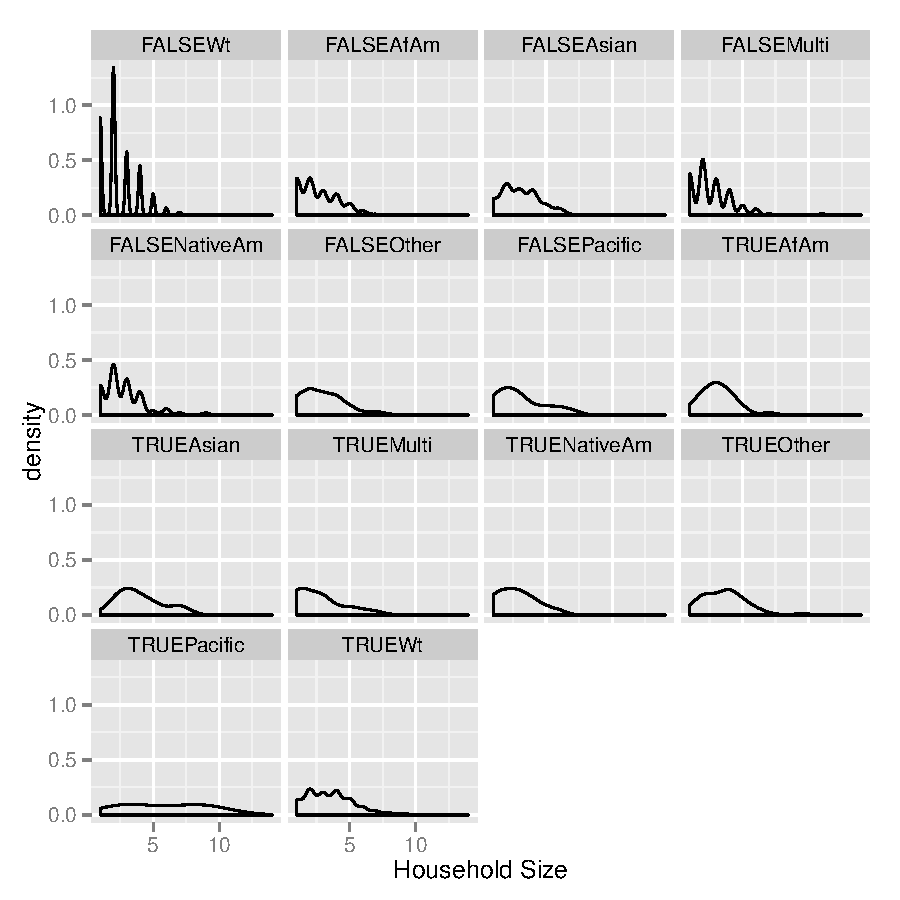
\includegraphics{DraftEdwardsWoods-007}
\end{center}
\end{figure}

Again, electric hot water service is more common in extreme rural areas and rental housing.  Figure \ref{fig:HeatFuel} shows a similar figure for heating fuel.  Non-Hispanic African Americans and Native Americans are more likely to have electric heat than non-Hispanic Caucasians, while Asian and Pacific Islanders have a large, ``Not applicable'', response category.   Again, Hispanic Caucasians are more likely to have electricity as their heating fuel than non-Hispanic Caucasians.

\begin{figure}[htbp]
\begin{center}
\caption{Heating Fuel by Race and Ethnicity}
\label{fig:HeatFuel}
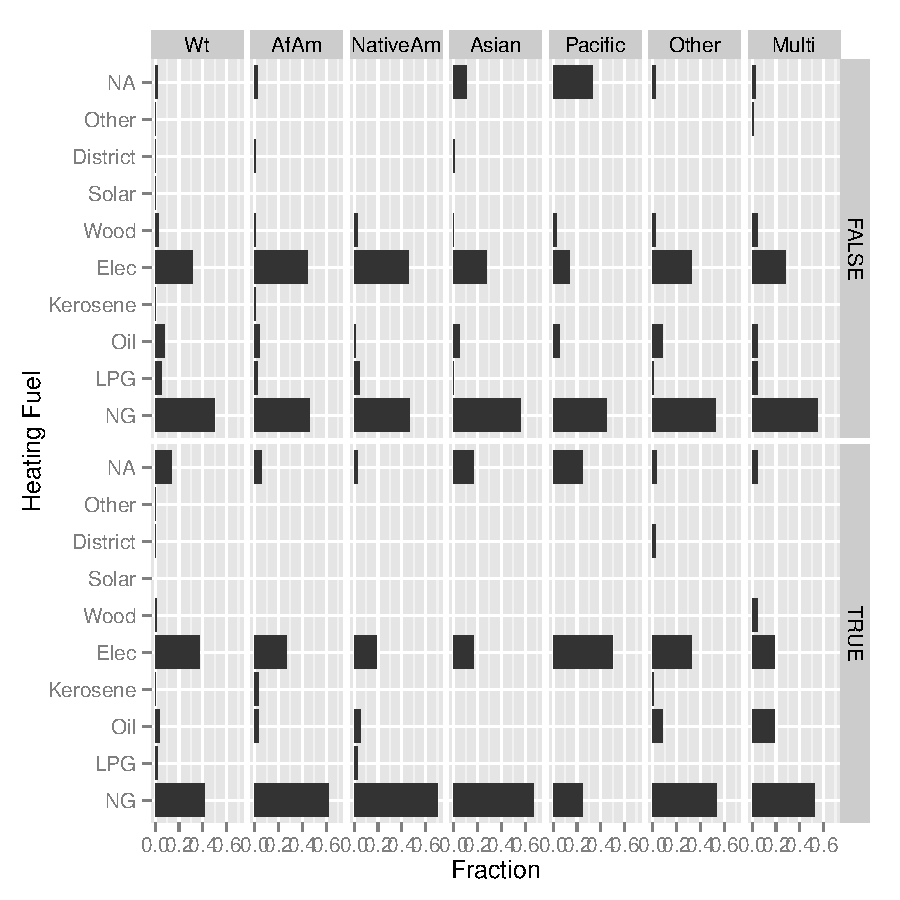
\includegraphics{DraftEdwardsWoods-008}
\end{center}
\end{figure}


Many of these different fuel choices can be partially explained by the locational choice made by the households.  Figure \ref{fig:HeatFuel} shows the climate type by race and ethnicity.  Non-Hispanic pacific islanders are more likely than non-Hispanic Caucasians to be in hot humid and marine environments and may explain the large number of not applicable responses for heating fuel.  Hispanic Caucasians are also more likely to live in hot dry/mixed dry or hot humid climes that the other groups.  While these climate types will still have some heating load, heating behavior and heating fuel is less likely to be a strong determinant of total electricity use.  Heating is just less an issue than cooling. 

\begin{figure}[htbp]
\begin{center}
\caption{Climate Type by Race and Ethnicity}
\label{fig:HeatFuel}
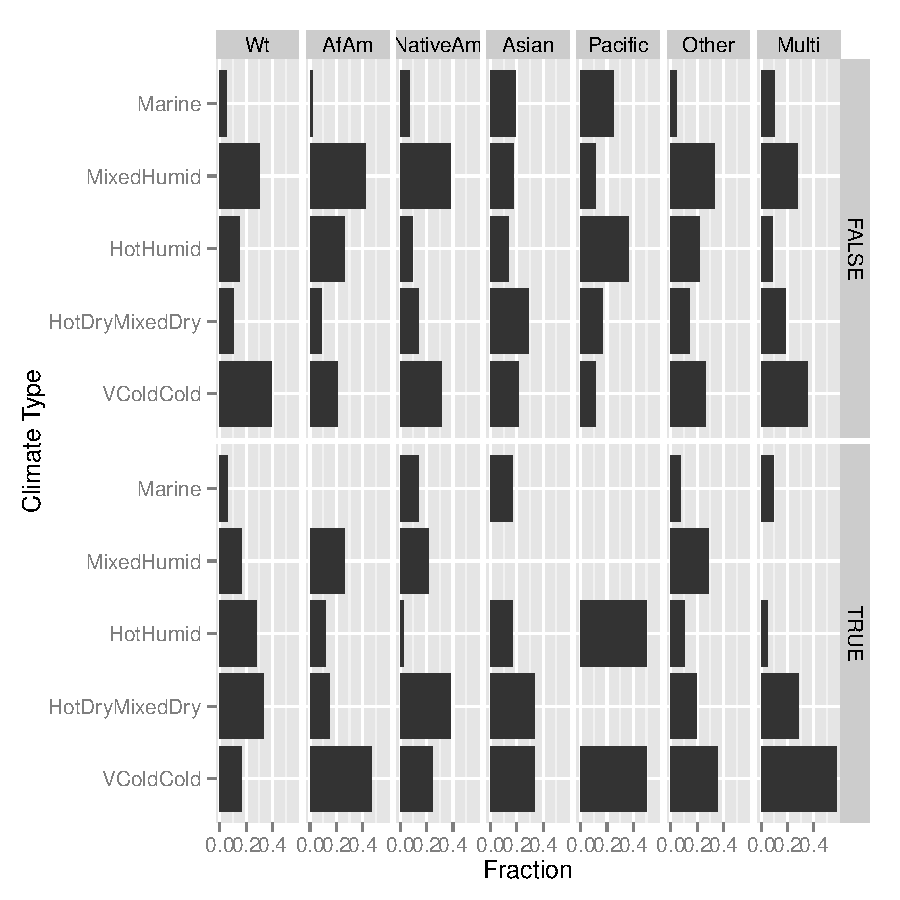
\includegraphics{DraftEdwardsWoods-009}
\end{center}
\end{figure}

There are also differences in the age of structure depending on both the race and ethnicity reported and if the household lives in an urban or rural area.  Figure \ref{fig:AgebyOwnRace} shows the distribution of the year the housing unit was built.  Columns indicate urban and rural households with the two left, $FALSE$, columns breaking out the non-Hispanic households and the right two, $TRUE$, showing the Hispanic households.  Rows are indicating the self-identified race.  There are several blank cells, where a smooth histogram is not possible because of the small number of observations.


\begin{figure}[htbp]
\begin{center}
\caption{Age of Structure by Rent/Own and Race/Ethnicity}
\label{fig:AgebyOwnRace}
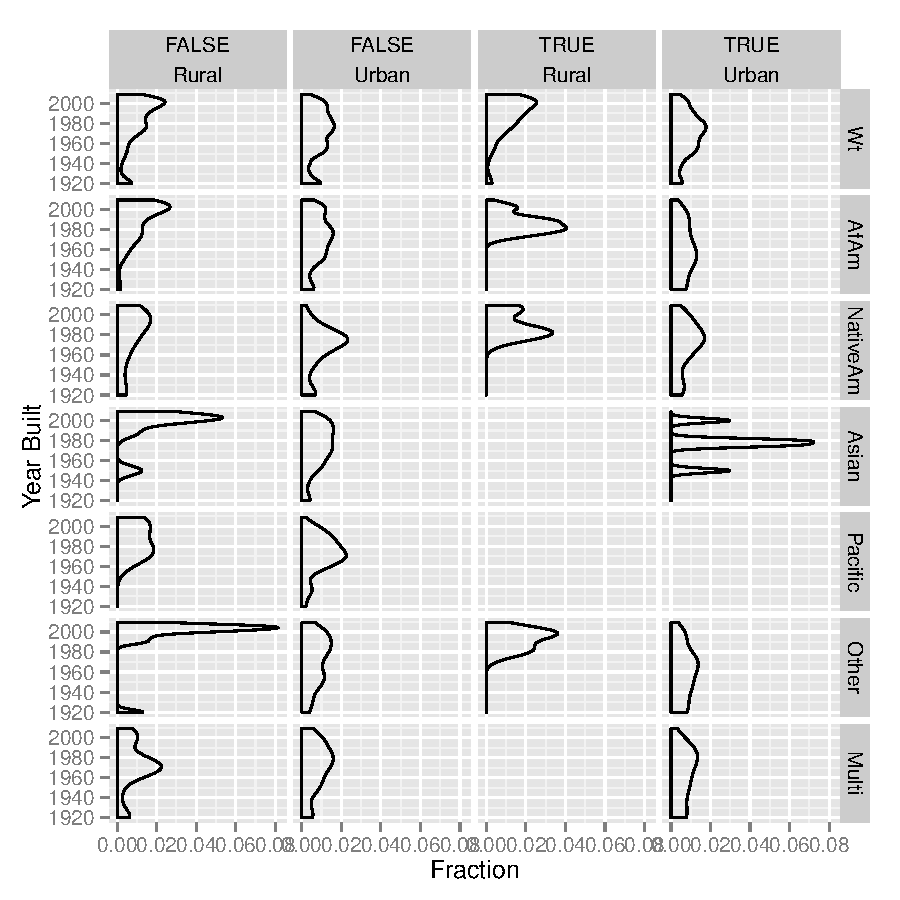
\includegraphics{DraftEdwardsWoods-010}
\end{center}
\end{figure}

What should be most apparent is that rural housing tends to be newer than urban housing.  Urban households have a modal construction date in the 1980s while the rural areas are more likely to have a model construction date in the 2000s.

These diagrams should lead one to the conclusion that important variables, such as location and fuel choice differ significantly across race and ethnicity and should not be treated, without great consideration, as exogenous.

\subsection{Differences in Reported Behavior}
%   
%   \begin{itemize}
%     \item Differnces in thermostat settings x
%     \item difference in cooking behavior x
%     \item difference in reported AC use
% 
%   \end{itemize}
%   
In spite of the evidence above that locational choice, tenure, and structure type decisions drive a great deal of energy use, there are still decisions, made after these choices that can be thought of as cultural differences.  Some of these may be regional preferences, for example the North East preference for higher winter indoor air temperatures, but there may be some true differences in behavior by race and ethnicity.

Consider figure \ref{fig:Meals} which shows the number of meals cooked in the home by race and ethnicity.  Non-Hispanic Caucasian household report a strong mode of one meal cooked in the house per day.  Non-Hispanic African Americans have a mode of one meal per week and Hispanic Caucasians have a mode of two a day.  Many of these differences can be attributed to differences in income across groups, but functional kitchens are virtually universal.


\begin{figure}
\begin{center}
\caption{Meals Cooked by Race and Ethnicity}
\label{fig:Meals}
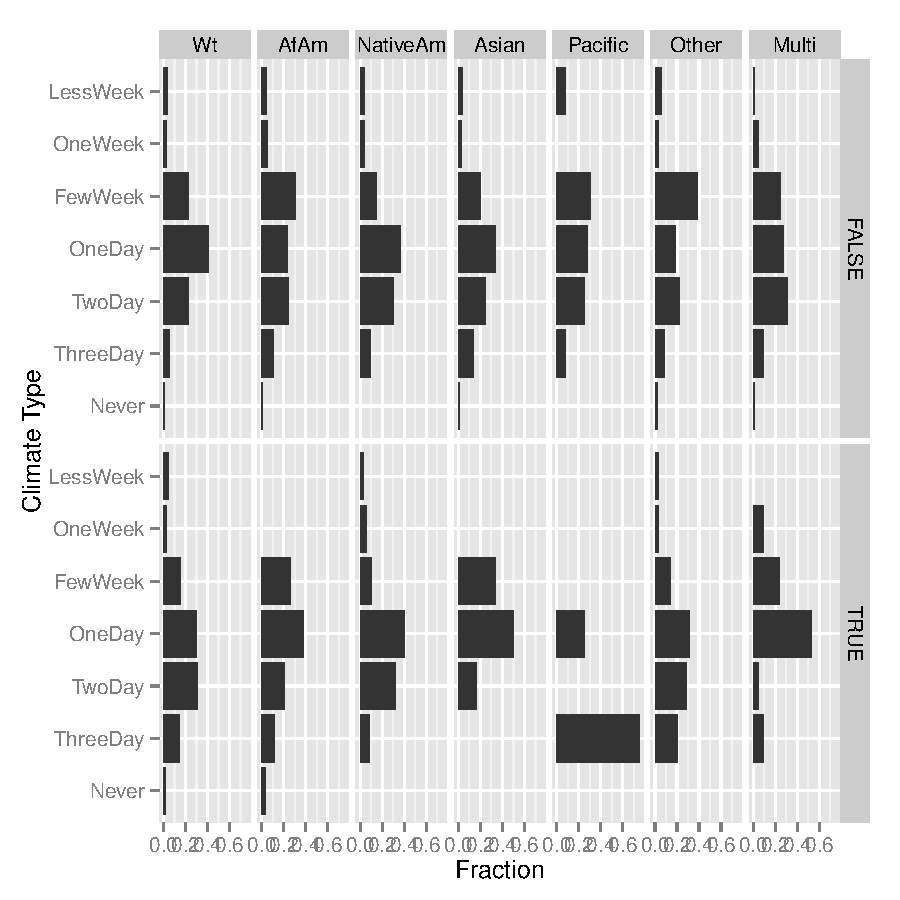
\includegraphics{DraftEdwardsWoods-011}
\end{center}
\end{figure}


The choice of thermostat setting is also made after the fact. The price of electricity, natural gas, square footage of the house, income, the presence of elderly residence can all have an effect on the choice of thermostat settings but these are all done after the equipment and location choices.  

Figure \ref{fig:TempHomeRace} shows box and whisker plots with notches for self-reported daytime thermostat settings in winter when someone is home.  The boxes show the 25\%-75\% interquartile range.  The bold mark shows the median and the notches give a visual test of a difference in medians for the groups.  If the notches overlap, you can not reject the null hypotheses that the thermostat settings are the same.  Note that for some of the cells with few observations, Hispanic Asians, the notches are wider than the interquartile range.

\begin{figure}
\begin{center}
\caption{Daytime Temp and Race/Ethnicity (Winter)}
\label{fig:TempHomeRace}
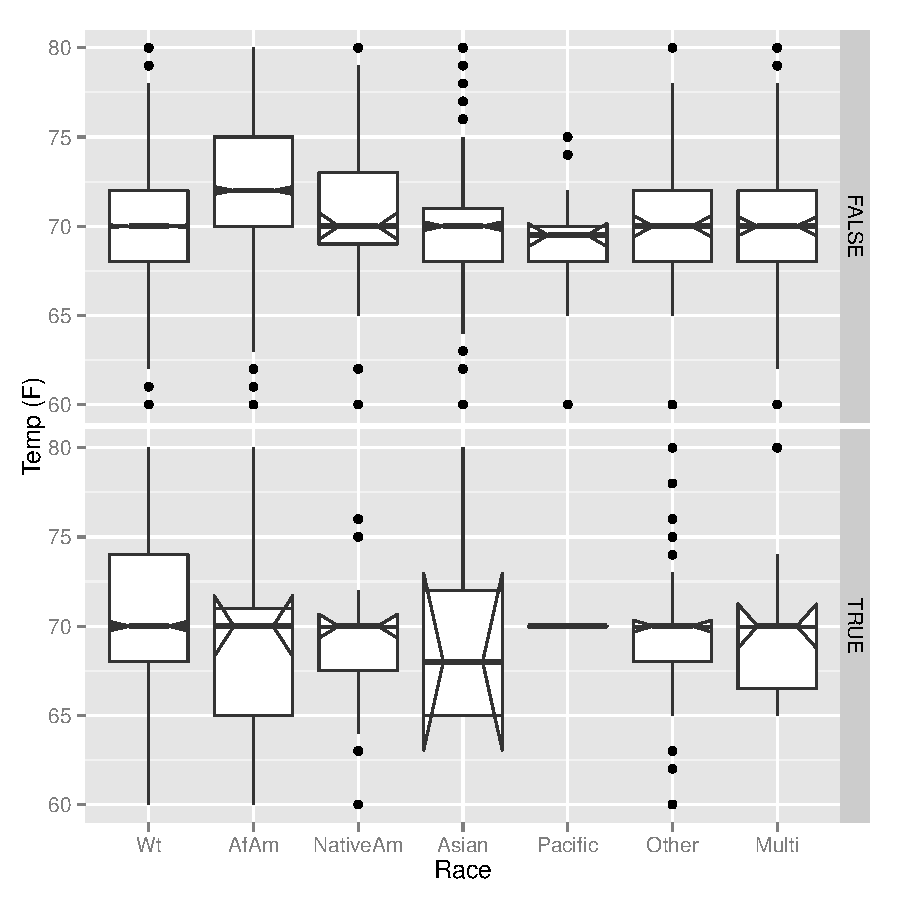
\includegraphics{DraftEdwardsWoods-012}
\end{center}
\end{figure}

The figure clearly shows that non-Hispanic African American households report a higher daytime winter thermostat setting than the other non-Hispanic groups.  This could be locational.  This could be cultural, but it is a behavioral difference that could make African American households more energy intensive in this end-use.

The effects of this higher thermostat setting may be offset by less electricity use for plug loads or hot water service or by having smaller residences, but it represents a different preference.

This difference in winter thermostat behavior follows through in summer thermostat preferences.  Figure \ref{fig:HomeRaceS} shows a summary for similar summer thermostat settings.  Note that non-Hispanic African Americans, Asian Americans and Native Americans all report lower summer thermostat settings than non-Hispanic and Hispanic Caucasian households.

\begin{figure}
\begin{center}
\caption{Daytime Temp Home by Race/Ethnicity (Summer)}
\label{fig:HomeRaceS}
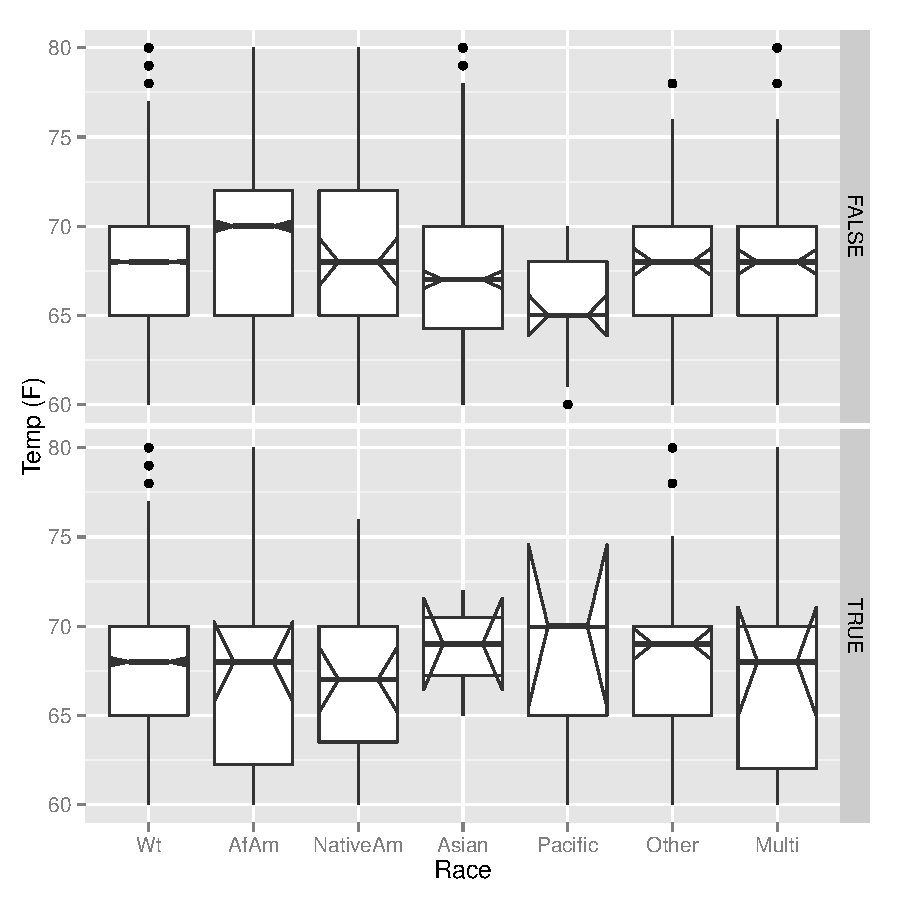
\includegraphics{DraftEdwardsWoods-013}
\end{center}
\end{figure}

*** TRANSITION TEXT NEEDED ***

\subsection{HUD Complaints as a Measure of Discrimination}\label{sec:WhyHUD}

Part of our hypothesis is that housing market discrimination is forcing some race and ethnicity groups into rental, older and poorer quality housing and that discrimination is leading to differences in electricity consumption that is currently being captured and interpreted as cultural differences.  Finding a state level index of housing market discrimination not easy.  While there are plenty of studies that show experimentally that housing market discrimination exists, an index that shows the extent of the discrimination is unavailable.

Until we construct a better index we are using a simple measure of the number of discrimination complaints filed with the U.S. Department of Housing and Urban Development as reported in their annual fair housing report \cite{HUD}.  There are problems with using complaints as an index of discrimination.

Complaints are only investigated if are reported to an agency that participates in the Federal Fair Housing Assistance program.  That program has a requirement that they enforce housing rights similar to the Fair Housing Act \cite[p. 17]{HUD}.  The data is accumulated in the Title Eight Automated Paperless Office Tracking System (TEAPOTS) system.  The majority of the complaints were because of disabilities but race is a close second in the number of complaints recorded \cite[p. 20]{HUD} with the most common violations being, ``Discriminatory Terms, Conditions, Privileges, Services, and Facilities in the Rental or Sale of Property''.

We treat complaints as evidence that there is housing market discrimination but it could be thought of as a compound event.  A complaint has as a prerequisite, an agency that enforces laws similar to the Fair Housing Act and the belief that a complaint will be acted upon.  You can have a low number of complaints if there is no discrimination but also because no one believes that a complaint is effective.  Until we construct a better index, which includes local law, field experiments similar to ***CITE*** this is as close as we can get to a statewide measure of housing market discrimination.
  
%   \begin{itemize}
%     \item trouble finding a good statewide index of housing discrimination
%     \item the HUD complaint measure
%     \item may be endogenous and be indicative of reduced discrimination
%   \end{itemize}
  
  
Table \ref{tab:HUDComplaints} shows the number of HUD complaints per 100,000 population by state.  States are aggregated the same way that location is reported in the RECS data set.  This means that, for example, states in the North East, Vermont, Rhode Island, New Hampshire, Connecticut and Maine share the same 20.50 complaints per 100,000, the highest reported complaint rate.  Other nearby states have a much lower rate, e.g., Pennsylvania with only 1.87 complaints per 100,000 population.

% latex table generated in R 3.0.1 by xtable 1.7-4 package
% Tue Apr  7 18:18:18 2015
\begin{table}[htbp]
\centering
\caption{HUD Complaints per 100,000 Population} 
\label{tab:HUDComplaints}
{\small
\begin{tabular}{llr}
  \hline
State & Population & Reports (per 100,000) \\ 
  \hline
Alabama & 4,677,464 & 7.50 \\ 
  Alaska & 688,125 & 13.01 \\ 
  Arizona & 6,499,377 & 3.68 \\ 
  Arkansas & 2,867,764 & 9.26 \\ 
  California & 36,580,371 & 3.03 \\ 
  Colorado & 4,935,213 & 1.97 \\ 
  Connecticut & 3,502,932 & 20.50 \\ 
  Delaware & 876,211 & 14.00 \\ 
  District of Columbia & 590,074 & 14.00 \\ 
  Florida & 18,423,878 & 3.93 \\ 
  Georgia & 9,697,838 & 2.06 \\ 
  Hawaii & 1,287,481 & 13.01 \\ 
  Idaho & 1,527,506 & 9.94 \\ 
  Illinois & 12,842,954 & 2.88 \\ 
  Indiana & 6,388,309 & 9.14 \\ 
  Iowa & 2,993,987 & 19.92 \\ 
  Kansas & 2,797,375 & 10.31 \\ 
  Kentucky & 4,287,931 & 7.50 \\ 
  Louisiana & 4,451,513 & 9.26 \\ 
  Maine & 1,319,691 & 20.50 \\ 
  Maryland & 5,658,655 & 14.00 \\ 
  Massachusetts & 6,543,595 & 4.51 \\ 
  Michigan & 10,002,486 & 4.97 \\ 
  Minnesota & 5,230,567 & 19.92 \\ 
  Mississippi & 2,940,212 & 7.50 \\ 
  Missouri & 5,956,335 & 4.99 \\ 
  Montana & 968,035 & 9.94 \\ 
  Nebraska & 1,781,949 & 10.31 \\ 
  Nevada & 2,615,772 & 5.08 \\ 
  New Hampshire & 1,321,872 & 20.50 \\ 
  New Jersey & 8,663,398 & 2.34 \\ 
  New Mexico & 1,986,763 & 5.08 \\ 
  New York & 19,467,789 & 4.60 \\ 
  North Carolina & 9,247,134 & 4.22 \\ 
  North Dakota & 641,421 & 19.92 \\ 
  Ohio & 11,528,072 & 9.14 \\ 
  Oklahoma & 3,644,025 & 9.26 \\ 
  Oregon & 3,782,991 & 13.01 \\ 
  Pennsylvania & 12,566,368 & 1.87 \\ 
  Rhode Island & 1,053,502 & 20.50 \\ 
  South Carolina & 4,503,280 & 4.22 \\ 
  South Dakota & 804,532 & 19.92 \\ 
  Tennessee & 6,240,456 & 2.61 \\ 
  Texas & 24,304,290 & 4.18 \\ 
  Utah & 2,727,343 & 9.94 \\ 
  Vermont & 621,049 & 20.50 \\ 
  Virginia & 7,795,424 & 2.03 \\ 
  Washington & 6,566,073 & 13.01 \\ 
  West Virginia & 1,814,873 & 14.00 \\ 
  Wisconsin & 5,627,610 & 1.81 \\ 
  Wyoming & 532,981 & 9.94 \\ 
   \hline
\end{tabular}
}
\end{table}
The fact that some states with a historical reputation for discrimination on the basis of race, Georgia and Illinois for example, have a very low complaint rate.  This highlights some of the difficulty in using HUD complaints as a measure of housing market discrimination.

\section{Conditional Demand Estimation}

  \subsection{Orthodox Results}
  
  \begin{itemize}
    \item Emphasize that we are making better use of race and ethnicity as a control with income than is common.
    \item We are not using the same estimation method as in RECS estimates of end use.  Our model is much simpler and does not use engineering estimates or significant non-linearity.
    \item Major end-uses are included but relatively unsophisticated.
    \item discuss the orthodox results.
  \end{itemize}
  
  
  
Modern conditional demand models of the kind commonly created as part of the process of data collection of large residential appliance and use surveys such as RECS, include a mix of engineering estimates, survey responses and analyst best estimates to produce energy end-use estimates.  For example, survey respondents will give an age range on the furnace they have installed, the square footage of the residence, and some indication of heating set points.  The analyst will assign a likely efficiency for the furnace based on the average of the age ranges and then estimate hours used based on set points, weather, and the reported thermostat settings.  This produces estimates that are closer to a Statistically Adjusted Engineering (SAE) model than what is normally regarded as a conditional demand model outside of the energy community.

Our model is based more on the traditional conditional demand models, and includes terms for electricity use contingent on: the age of the home, which is a proxy for building code requirements and insulation; the weather, in the form of Heating and Cooling degree days with a base temperature of 65F; Meals cooked at home, to indicate energy use related to food preparation; the number and age of refrigerators, a major end-use;  the number of and types of TVs and computers, as a proxy for major plug loads; the existence of a well pump; weather the residence has electric hot water service; the existence of pools and hot tubs as well as if they are electrically heated; the kind of windows installed, as another indication of shell quality; the number of people in the home; and finally the income, race and ethnicity of the residents.  


Model: Multinomial logit

As a point of clarity, surveys with questions not filled in were coded with 97, to differentiate between responses that were left blank and those where the value coded was not applicable.  For the purpose of this paper 97s were recoded to not and were dropped from the analysis.  

% The multinomial logit is first ran with owndwel as the dependent variable and the independent variables as follows: income, educ, race5, age_1, age_2.  The base chosen was that of house renters, represented here as the first category (see appendix).  Here, race5 represents whether the head of the household is white.  Running the multinomial logit with all raises included as independent variables proved problematic, and largely insignificant.  Ages of children were left separate in an attempt to model the difference between households with children of all ages and those with only young children.  Having only young children may represent households in starter homes who are not necessarily well established.  As well households with children over the age of eighteen are essentially ignored and treated as adults.  Another iteration of the model is also down removing the children variables and instead using resident count.
% The pseudo r-squared for the first model specified is 0.0912, which low it is important to bear in mind the problematic nature of interpreting pseudo r-squared values.  

Results:

The first and most likely indicator of home ownership within the structure type is income.  Here, we find in the results that the effect of income is statistically significant in each category accept the renting of townhomes.  Theory may suggest that, as mentioned earlier, row houses and townhomes in highly desirable neighborhoods especially historic neighborhoods are often rentals and as such might be rented by those with high incomes.  This question will remained unanswered within the scope of this study. 

 More importantly, the sign of the coefficient for income is positive for house ownership (approx. .22).  Continuing down the coefficients it is negative for townhouse rental (insignificant), positive for townhouse ownership, and the trend continues until that of mobile homes.  The income coefficient for mobile homes is negative for both rental and ownership, suggesting that a positive change in income has a negative effect on the probability of a household choosing a mobile home regardless if they are choosing to rent or buy.  It could be suggested that living in a mobile home is considered an inferior good, and households might choose to forego ownership or renting a mobile home in favor of choosing any other domicile.
 
The education variable is estimated, and is found to be statistically insignificant in the ownership of houses and the renting of townhouses and small complex apartment units.  Based on its coefficient, its value as an explanatory variable appears to be weak, yet as we go down the list of owndwel values the education coefficient moves from a positive to a negative at mobile homes. That is to say that here, education appears to have an effect mostly positive between the owndwel values of 3-8, and negative thereafter.

Race, the dummy for being white, is statistically significant everywhere except in the rental of apartments in large small complexes.  Note that for mobile homes the dummy for race takes on a value of approximately 1 and 1.57 for renters and owners respectively.  This would suggest, while not realistic probabilities, that overwhelmingly whites have a higher probability of choosing mobile homes in comparison to non-self-reporting whites.  Notably, no results of interest were found regarding the stereotype of Native-Americans dwelling in mobile homes within the data.  Also race in this case appears to be linked to ownership of homes in each of the categories, within the bootstrapped version of the model it is statistically significant in each of the ownership owndwel categories.  

% Age of children was found to be statistically significant in both variables largely.  The exceptions to the significance are in age_1, children under five for both large and small apartment complexes where households rent as well as the rental of mobile homes.  It is important to note that in each category the value of age_1 and age_2 coefficients is negative, which adds very little to our interpretations of the model.  Further, when we replace the children variables with that of resident count in the model we obtain a similar result where all coefficients are negative, and all statistically significant, in comparison to our base of house rental. 

When the model as specified first, is ran using a multinomial logit vce bootstrapping the results are slightly different with regards to children.  Now, while in places not statistically significant (see appendix) there does appear to be a trend towards the results are the same.  Further examination is needed.

%Fix latex ref
The parameter estimates of the full model can be found in appendix 
% \ref{OrthResults}
, partial results are shown in table 
% \ref{tab:ParOrthKWH}
.
  
% latex table generated in R 3.0.1 by xtable 1.7-4 package
% Tue Apr  7 18:18:19 2015
{\small
\begin{longtable}{rrrrr}
\caption{Orthodox kWh Model} \\ 
  \hline
 & Estimate & Std. Error & t value & Pr($>$$|$t$|$) \\ 
  \hline
Income & 0.0086 & 0.0016 & 5.3662 & 0.0000 \\ 
  Income:EthRaceFALSEAfAm & 0.0031 & 0.0027 & 1.1389 & 0.2548 \\ 
  Income:EthRaceFALSEAsian & -0.0243 & 0.0034 & -7.1646 & 0.0000 \\ 
  Income:EthRaceFALSEMulti & -0.0168 & 0.0069 & -2.4259 & 0.0153 \\ 
  Income:EthRaceFALSENativeAm & 0.0117 & 0.0123 & 0.9493 & 0.3425 \\ 
  Income:EthRaceFALSEOther & -0.0249 & 0.0083 & -2.9909 & 0.0028 \\ 
  Income:EthRaceFALSEPacific & -0.0163 & 0.0138 & -1.1807 & 0.2378 \\ 
  Income:EthRaceTRUEAfAm & -0.0120 & 0.0165 & -0.7271 & 0.4672 \\ 
  Income:EthRaceTRUEAsian & -0.0365 & 0.0454 & -0.8032 & 0.4219 \\ 
  Income:EthRaceTRUEMulti & -0.0291 & 0.0212 & -1.3745 & 0.1693 \\ 
  Income:EthRaceTRUENativeAm & -0.0187 & 0.0148 & -1.2599 & 0.2077 \\ 
  Income:EthRaceTRUEOther & -0.0262 & 0.0099 & -2.6335 & 0.0085 \\ 
  Income:EthRaceTRUEPacific & -0.0122 & 0.0380 & -0.3221 & 0.7474 \\ 
  Income:EthRaceTRUEWt & -0.0192 & 0.0031 & -6.2907 & 0.0000 \\ 
  StrTenureOwnSFDetached:TOTSQFT\_EN:HDD65 & 0.0001 & 0.0000 & 4.1043 & 0.0000 \\ 
  StrTenureOwnLgApartment:TOTSQFT\_EN:HDD65 & -0.0001 & 0.0001 & -0.9580 & 0.3381 \\ 
  StrTenureOwnMobile:TOTSQFT\_EN:HDD65 & 0.0004 & 0.0001 & 5.9838 & 0.0000 \\ 
  StrTenureOwnSFAttached:TOTSQFT\_EN:HDD65 & -0.0000 & 0.0000 & -0.5516 & 0.5812 \\ 
  StrTenureOwnSmApartment:TOTSQFT\_EN:HDD65 & 0.0000 & 0.0001 & 0.5438 & 0.5866 \\ 
  StrTenureRentLgApartment:TOTSQFT\_EN:HDD65 & -0.0002 & 0.0001 & -4.0031 & 0.0001 \\ 
  StrTenureRentMobile:TOTSQFT\_EN:HDD65 & 0.0004 & 0.0002 & 1.7633 & 0.0779 \\ 
  StrTenureRentSFAttached:TOTSQFT\_EN:HDD65 & 0.0000 & 0.0001 & 0.6010 & 0.5479 \\ 
  StrTenureRentSFDetached:TOTSQFT\_EN:HDD65 & 0.0000 & 0.0000 & 0.5515 & 0.5813 \\ 
  StrTenureRentSmApartment:TOTSQFT\_EN:HDD65 & -0.0001 & 0.0001 & -1.8580 & 0.0632 \\ 
  StrTenureOwnSFDetached:TOTSQFT\_EN:CDD65 & 0.0008 & 0.0000 & 19.2068 & 0.0000 \\ 
  StrTenureOwnLgApartment:TOTSQFT\_EN:CDD65 & -0.0002 & 0.0002 & -0.8168 & 0.4140 \\ 
  StrTenureOwnMobile:TOTSQFT\_EN:CDD65 & 0.0009 & 0.0001 & 7.3167 & 0.0000 \\ 
  StrTenureOwnSFAttached:TOTSQFT\_EN:CDD65 & 0.0006 & 0.0001 & 5.0127 & 0.0000 \\ 
  StrTenureOwnSmApartment:TOTSQFT\_EN:CDD65 & 0.0001 & 0.0003 & 0.4022 & 0.6875 \\ 
  StrTenureRentLgApartment:TOTSQFT\_EN:CDD65 & 0.0000 & 0.0001 & 0.3926 & 0.6946 \\ 
  StrTenureRentMobile:TOTSQFT\_EN:CDD65 & 0.0024 & 0.0004 & 6.3205 & 0.0000 \\ 
  StrTenureRentSFAttached:TOTSQFT\_EN:CDD65 & 0.0007 & 0.0002 & 4.0210 & 0.0001 \\ 
  StrTenureRentSFDetached:TOTSQFT\_EN:CDD65 & 0.0008 & 0.0001 & 9.2680 & 0.0000 \\ 
  StrTenureRentSmApartment:TOTSQFT\_EN:CDD65 & 0.0005 & 0.0002 & 2.8365 & 0.0046 \\ 
   \hline
\hline
\label{tab:OrthoKWHLimited}
\end{longtable}
}
The top parameter, Income, shows the estimate for annual kWh per dollar of income for a household headed by a non-Hispanic Caucasian.  The remaining income related variables show the deviations from this case for Hispanic headed households, labeled TRUE in the table, and by the other self reported races.  Note that in all cases, with the exception of non-Hispanic Native Americans, the parameter estimates show less electricity used than non-Hispanic Caucasian households.  Only a few of these differences are statistically significant, non-Hispanic Asian and multi-ethnic households, as well as Hispanic Caucasian households and households that reported some other race.

The remaining items shown in the table show the electricity use per square foot for each of the structure types, e.g., Single Family Detached, and tenure, i.e., Rent or Own, per annual heating and cooling degree days.  Aside from the negative and significant estimate for the heating load in large Rented apartments, the results are unremarkable. 

\subsection{Endogenizing Structure and Other Variables}\label{sec:SingleEq}

Treating structure type and square footage as endogenous is our first step in estimating conditional demand for many end uses treating the choice of things like, EnergyStar appliances, refrigerator size and design.  The current standard, treating these as exogenous drivers of energy use biases or estimates of energy use in unknown ways.

Focusing on tenure, i.e., the decision to own or rent, structure and square footage decisions allows us to see if other housing market institutions are driving energy use differently depending on ethnicity.  At this early stage of research we are focusing only on these major drivers but we can expand the analysis to other choices including clothes washing, hot water service and other large energy drivers.

As stated in section \ref{sec:WhyHUD}, using HUD complaints as a measure of housing market discrimination based on race and ethnicity is less than optimal measure, but at this early stage is an adequate measure to determine the scale of the effect.  


Table 
% \ref{tab:OrthoSQFTLimited} 
shows only the discrimination related results for our model of square footage.  Full results can be seen in appendix 
% \ref{OrthResults}
.   Note that the square footage model includes structure type and tenure as an exogenous variable.  This model of square footage will be included later as part of a system estimation of electricity use.   

The key discrimination variable, reporttot, is the count of complaints received by HUD per 100,000 people in the state where the household is located. We interacted this variable with race and ethnicity to allow for different effects  groups but we do not allow the discrimination to vary by state. Note that the effects of HUD reports on square footage are rarely significant, only strongly significant for Hispanic Caucasian households.  In this case incidences of HUD complaints per 100,000 of state population results in a reduction in the square footage for Caucasian Hispanics by 22.73 square feet.

This model is in general not very good at explaining square footage; the adjusted $R^2$ is only $.3897$.  This weakness will plague us later when we jointly estimate this model with structure type, tenure and electricity use, but illustrates one of the ways we can endogenize the choices that lead to electricity consumption.


% \begin{itemize}
%   \item explain the logic behind the making both sqft and structure tenure endogenous.
%   \item primarily that sqft may be related to quality of houseing, newer structures
% \end{itemize}



While the impact of housing market discrimination has some effect on the size of residences, the effects on the ownership and structure type decision is expected to be more dramatic.  Housing market discrimination can be expected to push some people away from owned property and into the rental market, which is rife with split incentives for conservation and energy efficiency investments.  

Discrimination can also push some households into structure types, where even when owned, that have significant split incentives for energy efficiency investments.  Take, for example, small and large apartment buildings.  While the householder may have control over some appliances, the building shell and some of the heating and cooling equipment decisions are made by others.  

Our model of structure type and tenure includes categories for both owned and rented: Large Apartments, Small Apartments, Mobile Homes, Single Family Detached, and Single Family Attached.  We explain the joint tenure and structure type with: the square footage of the structure, if the household receives rental assistance, income, number of people in the household, education level of the head of household, the HUD reports per 100,000 in that state and whether the household is in a rural or urban location.  As in the square footage model, HUD reports are interacted with the race and ethnicity variables to allow for separate discrimination effects for each.


All parameter estimates for the models are statistically significant at the 1\% level, with the exception of the income variable which is highly correlated with the education variables, and are displayed in appendix. 
% \ref{OrthResults}. 


%Fix the Latex part of this.
Since all the parameters are statistically significant it is easier to show the effects of our measure of housing market discrimination on the probability of each structure and tenure choice for the race and ethnicity combinations.  The HUD reports run from 1.81249 complaints per 100,000 to 20.496 complaints per 100,000.  Figure 
% \ref{fig:HUDOnChoice} 
shows the reaction to HUD complaints over the 1 to 21 complaint range.


% 
% \begin{figure}
% \begin{center}\label{fig:HUDOnChoice}
% 
% <<echo=false,fig=TRUE>>=
% # Need to figure this figure out.  It may be very complex
% 
% @
% \end{center}
% \end{figure}

***Lots of explanation goes here***




  \subsection{System Estimation}

The single equation results discussed in section \ref{sec:SingleEq} show strong promise for endogenizing some of the decisions made about structure and equipment within the conditional demand model as well as the potential importance of housing market discrimination in structure choice.  In this section we treat square footage, tenure and structure type as endogenous and estimate estimate the electricity, structure/tenure, and square footage model as a system.

It is unclear how this can be accomplished in a full information, so we chose a two-stage least squares technique, estimating first the square footage model, then using forecasted values to estimate tenure and structure type model.  Forecasts from that model were used to resestimate and produce a new round of forecasts for the square footage model.  Both the forecasts of the structure tenure model and square footage model were then used to estimate the conditional demand model.

This should produce consistent results but the variance of the parameter estimates are biased.  It is unclear how to make the usual corrections to the variance of the parameter estimates given that the structure and tenure model is estimated as a multinomial logit.  The best alternative is to bootstrap the system.  There are a few caveats.

First, the bootstrap sampling is stratified so that all parameter estimates in all models can be estimated.  This is particularly important in the structure and tenure model.  We had to ensure enough observations of the rare endogenous cells, rented mobile homes being the most restricted, and exogenous variables, e.g., Hispanic Pacific Islanders.  This was accomplished by simple rejection sampling rather than assigning different probabilities of selection to each of the cells.

Second, we did not censor non-positive square footage forecasts.  The square footage model is weaker than expected and it was quite possible to have negative forecasts.  Alternative models, such as Tobit, would not be effective, but we are considering transformations of square footage as we move forward.  

Finally, only 400 bootstrap replicates were evaluated.  This is usually enough to produce adequate estimates of the standard deviations of the parameter estimates in the electricity model but insufficient for BCa, percentile, or even basic bootstrap confidence intervals. 

% \begin{itemize}
%   \item results are bootstrapped 400 times for standard deviation estimates.  More can be done.
%   \item probablities of structure type rather than forecast were used.
%   \item no censoring for square footage less than zero.
%   \item boot strap samples were restricted to samples that allowed for all parameters to be estimated.
% \end{itemize}




The full set of parameter estimates for the electricity model can be found in the appendix.  We will focus on a subset of the parameter estimates, focusing on the effects of race and ethnicity separately and the effects of the other endogenous variables, structure and tenure and square footage.

% latex table generated in R 3.0.1 by xtable 1.7-4 package
% Tue Apr  7 18:18:20 2015
{\small
\begin{longtable}{rrrrl}
\caption{System Estimation of kWh Model: Race and Ethnicity} \\ 
  \hline
 & Estimate & Std. Error & t value & Sig \\ 
  \hline
Income:EthRaceFALSEAfAm & 0.0052 & 0.0029 & 1.7791 &   \\ 
  Income:EthRaceFALSEAsian & -0.0230 & 0.0035 & -6.4831 & *** \\ 
  Income:EthRaceFALSEMulti & -0.0157 & 0.0057 & -2.7584 & * \\ 
  Income:EthRaceFALSENativeAm & 0.0092 & 0.0211 & 0.4382 &   \\ 
  Income:EthRaceFALSEOther & -0.0237 & 0.0082 & -2.9038 & * \\ 
  Income:EthRaceFALSEPacific & -0.0129 & 0.0230 & -0.5625 &   \\ 
  Income:EthRaceTRUEAfAm & -0.0173 & 0.0139 & -1.2454 &   \\ 
  Income:EthRaceTRUEAsian & -0.0375 & 0.0101 & -3.7155 & ** \\ 
  Income:EthRaceTRUEMulti & -0.0331 & 0.0192 & -1.7208 &   \\ 
  Income:EthRaceTRUENativeAm & -0.0163 & 0.0107 & -1.5276 &   \\ 
  Income:EthRaceTRUEOther & -0.0274 & 0.0080 & -3.4318 & ** \\ 
  Income:EthRaceTRUEPacific & -0.0240 & 0.0659 & -0.3647 &   \\ 
  Income:EthRaceTRUEWt & -0.0185 & 0.0033 & -5.5782 & *** \\ 
   \hline
\hline
\label{tab:SystemKWHEthnicity}
\end{longtable}
}
Table 
% \ref{tab:SystemKWHEthnicity}
shows similarities with the results from the orthodox electricity model.  Non-Hispanic Asians, and Hispanic Caucasians and Hispanic heads of households that identify as some other race all show lower electricity use per dollar of income.   This is consistent in sign with the parameter estimates in table 
% \ref{tab:ParOrthKWH}
, but the statistically significant deviations from non-Hispanic Caucasians for non Hispanic multi-ethnic heads of household has vanished.  The scale of the significant parameter estimates are also roughly the same magnitude but attenuated towards zero.

% latex table generated in R 3.0.1 by xtable 1.7-4 package
% Tue Apr  7 18:18:20 2015
{\small
\begin{longtable}{rrrrl}
\caption{System Estimation of kWh Model: Square Footage} \\ 
  \hline
 & Estimate & Std. Error & t value & Sig \\ 
  \hline
PSQFT:OwnSFDetached:HDD65 & 0.0001 & 0.0000 & 4.4109 & *** \\ 
  PSQFT:HDD65:OwnLgApartment & 0.0000 & 0.0001 & 0.8450 &   \\ 
  PSQFT:HDD65:OwnMobile & 0.0004 & 0.0001 & 4.6205 & *** \\ 
  PSQFT:HDD65:OwnSFAttached & 0.0000 & 0.0000 & 1.3603 &   \\ 
  PSQFT:HDD65:OwnSmApartment & 0.0001 & 0.0000 & 1.1709 &   \\ 
  PSQFT:HDD65:RentLgApartment & -0.0001 & 0.0000 & -1.3292 &   \\ 
  PSQFT:HDD65:RentMobile & 0.0005 & 0.0003 & 2.0238 &   \\ 
  PSQFT:HDD65:RentSFAttached & 0.0001 & 0.0001 & 1.0923 &   \\ 
  PSQFT:HDD65:RentSFDetached & 0.0001 & 0.0000 & 1.7233 &   \\ 
  PSQFT:HDD65:RentSmApartment & -0.0000 & 0.0000 & -0.2465 &   \\ 
  PSQFT:OwnSFDetached:CDD65 & 0.0007 & 0.0000 & 16.3870 & *** \\ 
  PSQFT:OwnLgApartment:CDD65 & 0.0000 & 0.0002 & 0.2207 &   \\ 
  PSQFT:OwnMobile:CDD65 & 0.0011 & 0.0002 & 6.7660 & *** \\ 
  PSQFT:OwnSFAttached:CDD65 & 0.0005 & 0.0001 & 5.3085 & *** \\ 
  PSQFT:OwnSmApartment:CDD65 & 0.0003 & 0.0002 & 1.8671 &   \\ 
  PSQFT:RentLgApartment:CDD65 & 0.0003 & 0.0001 & 2.5551 & . \\ 
  PSQFT:RentMobile:CDD65 & 0.0020 & 0.0009 & 2.2066 &   \\ 
  PSQFT:RentSFAttached:CDD65 & 0.0009 & 0.0002 & 4.9470 & *** \\ 
  PSQFT:RentSFDetached:CDD65 & 0.0008 & 0.0001 & 8.8123 & *** \\ 
  PSQFT:RentSmApartment:CDD65 & 0.0005 & 0.0001 & 3.5753 & ** \\ 
   \hline
\hline
\label{tab:SystemKWHSQFT}
\end{longtable}
}
Table 
% \ref{tab:SystemKWHSQFT}
shows the relationship between heating and cooling degree days per square foot on electricity use for each of the tenure and structure type combinations.  These results are particularly troublesome because heating and cooling degree days, in conjunction with square footage, are one of the most reliable explanatory variables for electricity use.  Space heating and cooling are two major end-uses in most households.  The parameter estimates show that these reliable explanatory variables are only significant in a few rare cases.  There is a strong relationship heating and cooling degree days for owned single family detached structures, but only rented mobile homes show statistically significant reactions to heating loads and only large apartments, owned or rented, for cooling loads.

This is very strong evidence that our square footage choice model needs improvement if it will be used as part of this electricity consumption system. 

\section{Summary and Conclusions}

The model set out to provide some explanation of housing choices based on relevant variables.  In doing so it is apparent that income places a significant role in the formation of house choices both to own/rent and what type of structure is chosen.  Further education played a less significant role than anticipated, thought it could be said that the role of education is actually channeled through income.  As such its placement in the model is suspect in its current form.

The race variable appears to suggest that whites tend towards ownership of their homes, and that whites are more likely to live in mobile homes than other races.  Further examination of race within this model framework would be an interesting and possibly useful endeavor. 

The model would likely benefit by an expansion of the explanatory variables in an effort to provide a better fit.  It is relevant to point out that this is a model in progress whose ultimate goal is that of modeling household characteristics on energy consumption.


As well, the location of a structure type to needs such as: employment, school districts, entertainment, and public services etc., may play a role in choice of homes.  This last point is not considered within the scope of the model.  


\cite{boot}
\nocite{*}
\bibliographystyle{plain} 
\bibliography{FullBib}

\appendix
\section{Full Regression Results}\label{OrthResults}


% latex table generated in R 3.0.1 by xtable 1.7-4 package
% Tue Apr  7 18:18:20 2015
{\small
\begin{longtable}{rrrrr}
\caption{Orthodox kWh Model} \\ 
  \hline
 & Estimate & Std. Error & t value & Pr($>$$|$t$|$) \\ 
  \hline
(Intercept) & 2181.1197 & 1792.3947 & 1.22 & 0.2237 \\ 
  ElecMealsThreeDay & 1338.6588 & 297.7217 & 4.50 & 0.0000 \\ 
  ElecMealsTwoDay & 1644.3185 & 185.0764 & 8.88 & 0.0000 \\ 
  ElecMealsOneDay & 1685.3404 & 159.1570 & 10.59 & 0.0000 \\ 
  ElecMealsFewWeek & 1451.1356 & 183.7584 & 7.90 & 0.0000 \\ 
  ElecMealsOneWeek & 1726.8842 & 406.3322 & 4.25 & 0.0000 \\ 
  ElecMealsLessWeek & 992.8116 & 424.8594 & 2.34 & 0.0195 \\ 
  NUMFRIG & 1574.9574 & 120.8432 & 13.03 & 0.0000 \\ 
  AgeFridge2to4Years & 49.6457 & 195.1174 & 0.25 & 0.7992 \\ 
  AgeFridge5to9Years & 312.9075 & 183.1243 & 1.71 & 0.0875 \\ 
  AgeFridge20PlusYears & 282.4503 & 328.6753 & 0.86 & 0.3902 \\ 
  AgeFridge10to14Years & 392.2705 & 207.4396 & 1.89 & 0.0587 \\ 
  AgeFridge15to19Years & 3.4299 & 283.6629 & 0.01 & 0.9904 \\ 
  NUMPC & 345.0370 & 64.3126 & 5.37 & 0.0000 \\ 
  TIMEON1OneTo3Hrs & -142.2026 & 160.6198 & -0.89 & 0.3760 \\ 
  TIMEON1ThreeTo6Hrs & -5.9463 & 186.4186 & -0.03 & 0.9746 \\ 
  TIMEON1SixTo10Hrs & 224.2810 & 239.0840 & 0.94 & 0.3482 \\ 
  TIMEON1Gr10 & 823.2281 & 214.7291 & 3.83 & 0.0001 \\ 
  WELLPUMPTRUE & 1501.4018 & 183.5027 & 8.18 & 0.0000 \\ 
  ElecWaterSmall & 4421.9192 & 256.3522 & 17.25 & 0.0000 \\ 
  ElecWaterMed & 4658.3555 & 163.9114 & 28.42 & 0.0000 \\ 
  ElecWaterLrg & 5809.5827 & 189.7584 & 30.62 & 0.0000 \\ 
  ElecWaterTankless & 3251.7517 & 755.3718 & 4.30 & 0.0000 \\ 
  SWIMPOOLTRUE & 3228.7285 & 222.3292 & 14.52 & 0.0000 \\ 
  ElecPoolTRUE & 4604.1557 & 837.0574 & 5.50 & 0.0000 \\ 
  RECBATHTRUE & 1013.4653 & 426.3413 & 2.38 & 0.0175 \\ 
  ElecTubTRUE & 1218.8041 & 486.6005 & 2.50 & 0.0123 \\ 
  NHSLDMEM & 952.0720 & 42.5506 & 22.38 & 0.0000 \\ 
  Income & 0.0086 & 0.0016 & 5.37 & 0.0000 \\ 
  TVONWD1LessHour:TVTYPE1Standard & -3266.1101 & 1800.2730 & -1.81 & 0.0697 \\ 
  TVONWD1OneTo3Hrs:TVTYPE1Standard & -3010.1255 & 1775.5111 & -1.70 & 0.0900 \\ 
  TVONWD1ThreeTo6Hrs:TVTYPE1Standard & -2516.9211 & 1772.6818 & -1.42 & 0.1557 \\ 
  TVONWD1SixTo10Hrs:TVTYPE1Standard & -1794.7156 & 1778.9345 & -1.01 & 0.3131 \\ 
  TVONWD1Gr10:TVTYPE1Standard & -1290.6207 & 1784.9518 & -0.72 & 0.4697 \\ 
  TVONWD1LessHour:TVTYPE1LCD & -2896.8097 & 1807.2466 & -1.60 & 0.1090 \\ 
  TVONWD1OneTo3Hrs:TVTYPE1LCD & -2313.1891 & 1773.9814 & -1.30 & 0.1923 \\ 
  TVONWD1ThreeTo6Hrs:TVTYPE1LCD & -1955.8036 & 1770.9445 & -1.10 & 0.2695 \\ 
  TVONWD1SixTo10Hrs:TVTYPE1LCD & -1593.9919 & 1777.1898 & -0.90 & 0.3698 \\ 
  TVONWD1Gr10:TVTYPE1LCD & -485.7205 & 1785.6404 & -0.27 & 0.7856 \\ 
  TVONWD1LessHour:TVTYPE1Plasma & -1497.7500 & 1988.0024 & -0.75 & 0.4512 \\ 
  TVONWD1OneTo3Hrs:TVTYPE1Plasma & -1664.7504 & 1800.8346 & -0.92 & 0.3553 \\ 
  TVONWD1ThreeTo6Hrs:TVTYPE1Plasma & -2001.8306 & 1788.6852 & -1.12 & 0.2631 \\ 
  TVONWD1SixTo10Hrs:TVTYPE1Plasma & -940.8541 & 1815.7684 & -0.52 & 0.6044 \\ 
  TVONWD1Gr10:TVTYPE1Plasma & 418.9083 & 1846.1024 & 0.23 & 0.8205 \\ 
  TVONWD1LessHour:TVTYPE1Projection & -2094.9059 & 2146.9297 & -0.98 & 0.3292 \\ 
  TVONWD1OneTo3Hrs:TVTYPE1Projection & -1639.6049 & 1851.1064 & -0.89 & 0.3758 \\ 
  TVONWD1ThreeTo6Hrs:TVTYPE1Projection & -2152.3377 & 1812.9470 & -1.19 & 0.2352 \\ 
  TVONWD1SixTo10Hrs:TVTYPE1Projection & -925.1902 & 1837.7040 & -0.50 & 0.6147 \\ 
  TVONWD1Gr10:TVTYPE1Projection & 1530.2305 & 1911.2140 & 0.80 & 0.4234 \\ 
  TVONWD1LessHour:TVTYPE1LED & -4513.1128 & 2901.1001 & -1.56 & 0.1198 \\ 
  TVONWD1OneTo3Hrs:TVTYPE1LED & -1678.7884 & 2013.2805 & -0.83 & 0.4044 \\ 
  TVONWD1ThreeTo6Hrs:TVTYPE1LED & -2106.7446 & 1923.5912 & -1.10 & 0.2735 \\ 
  TVONWD1SixTo10Hrs:TVTYPE1LED & -3418.0720 & 2390.7609 & -1.43 & 0.1528 \\ 
  TOTSQFT\_EN:TYPEGLASSSinglePane & -0.1921 & 0.1586 & -1.21 & 0.2259 \\ 
  TOTSQFT\_EN:TYPEGLASSDoublePane & -0.0336 & 0.1540 & -0.22 & 0.8271 \\ 
  TOTSQFT\_EN:TYPEGLASSTriplePane & 0.0093 & 0.2093 & 0.04 & 0.9644 \\ 
  Income:EthRaceFALSEAfAm & 0.0031 & 0.0027 & 1.14 & 0.2548 \\ 
  Income:EthRaceFALSEAsian & -0.0243 & 0.0034 & -7.16 & 0.0000 \\ 
  Income:EthRaceFALSEMulti & -0.0168 & 0.0069 & -2.43 & 0.0153 \\ 
  Income:EthRaceFALSENativeAm & 0.0117 & 0.0123 & 0.95 & 0.3425 \\ 
  Income:EthRaceFALSEOther & -0.0249 & 0.0083 & -2.99 & 0.0028 \\ 
  Income:EthRaceFALSEPacific & -0.0163 & 0.0138 & -1.18 & 0.2378 \\ 
  Income:EthRaceTRUEAfAm & -0.0120 & 0.0165 & -0.73 & 0.4672 \\ 
  Income:EthRaceTRUEAsian & -0.0365 & 0.0454 & -0.80 & 0.4219 \\ 
  Income:EthRaceTRUEMulti & -0.0291 & 0.0212 & -1.37 & 0.1693 \\ 
  Income:EthRaceTRUENativeAm & -0.0187 & 0.0148 & -1.26 & 0.2077 \\ 
  Income:EthRaceTRUEOther & -0.0262 & 0.0099 & -2.63 & 0.0085 \\ 
  Income:EthRaceTRUEPacific & -0.0122 & 0.0380 & -0.32 & 0.7474 \\ 
  Income:EthRaceTRUEWt & -0.0192 & 0.0031 & -6.29 & 0.0000 \\ 
  StrTenureOwnSFDetached:TOTSQFT\_EN:HDD65 & 0.0001 & 0.0000 & 4.10 & 0.0000 \\ 
  StrTenureOwnLgApartment:TOTSQFT\_EN:HDD65 & -0.0001 & 0.0001 & -0.96 & 0.3381 \\ 
  StrTenureOwnMobile:TOTSQFT\_EN:HDD65 & 0.0004 & 0.0001 & 5.98 & 0.0000 \\ 
  StrTenureOwnSFAttached:TOTSQFT\_EN:HDD65 & -0.0000 & 0.0000 & -0.55 & 0.5812 \\ 
  StrTenureOwnSmApartment:TOTSQFT\_EN:HDD65 & 0.0000 & 0.0001 & 0.54 & 0.5866 \\ 
  StrTenureRentLgApartment:TOTSQFT\_EN:HDD65 & -0.0002 & 0.0001 & -4.00 & 0.0001 \\ 
  StrTenureRentMobile:TOTSQFT\_EN:HDD65 & 0.0004 & 0.0002 & 1.76 & 0.0779 \\ 
  StrTenureRentSFAttached:TOTSQFT\_EN:HDD65 & 0.0000 & 0.0001 & 0.60 & 0.5479 \\ 
  StrTenureRentSFDetached:TOTSQFT\_EN:HDD65 & 0.0000 & 0.0000 & 0.55 & 0.5813 \\ 
  StrTenureRentSmApartment:TOTSQFT\_EN:HDD65 & -0.0001 & 0.0001 & -1.86 & 0.0632 \\ 
  StrTenureOwnSFDetached:TOTSQFT\_EN:CDD65 & 0.0008 & 0.0000 & 19.21 & 0.0000 \\ 
  StrTenureOwnLgApartment:TOTSQFT\_EN:CDD65 & -0.0002 & 0.0002 & -0.82 & 0.4140 \\ 
  StrTenureOwnMobile:TOTSQFT\_EN:CDD65 & 0.0009 & 0.0001 & 7.32 & 0.0000 \\ 
  StrTenureOwnSFAttached:TOTSQFT\_EN:CDD65 & 0.0006 & 0.0001 & 5.01 & 0.0000 \\ 
  StrTenureOwnSmApartment:TOTSQFT\_EN:CDD65 & 0.0001 & 0.0003 & 0.40 & 0.6875 \\ 
  StrTenureRentLgApartment:TOTSQFT\_EN:CDD65 & 0.0000 & 0.0001 & 0.39 & 0.6946 \\ 
  StrTenureRentMobile:TOTSQFT\_EN:CDD65 & 0.0024 & 0.0004 & 6.32 & 0.0000 \\ 
  StrTenureRentSFAttached:TOTSQFT\_EN:CDD65 & 0.0007 & 0.0002 & 4.02 & 0.0001 \\ 
  StrTenureRentSFDetached:TOTSQFT\_EN:CDD65 & 0.0008 & 0.0001 & 9.27 & 0.0000 \\ 
  StrTenureRentSmApartment:TOTSQFT\_EN:CDD65 & 0.0005 & 0.0002 & 2.84 & 0.0046 \\ 
   \hline
\hline
\label{tab:OrthoKWHFull}
\end{longtable}
}
% latex table generated in R 3.0.1 by xtable 1.7-4 package
% Tue Apr  7 18:18:20 2015
{\small
\begin{longtable}{rrrrr}
\caption{Orthodox Square Foot Model} \\ 
  \hline
 & Estimate & Std. Error & t value & Pr($>$$|$t$|$) \\ 
  \hline
(Intercept) & 1944.2850 & 75.4800 & 25.76 & 0.0000 \\ 
  RENTHELPTRUE & 182.1575 & 82.5453 & 2.21 & 0.0274 \\ 
  StrTenureOwnLgApartment & -1374.2383 & 67.6666 & -20.31 & 0.0000 \\ 
  StrTenureOwnMobile & -1095.7710 & 47.1356 & -23.25 & 0.0000 \\ 
  StrTenureOwnSFAttached & -493.4629 & 52.5900 & -9.38 & 0.0000 \\ 
  StrTenureOwnSmApartment & -776.3654 & 87.1475 & -8.91 & 0.0000 \\ 
  StrTenureRentLgApartment & -1393.2440 & 30.1078 & -46.28 & 0.0000 \\ 
  StrTenureRentMobile & -1202.7143 & 95.8133 & -12.55 & 0.0000 \\ 
  StrTenureRentSFAttached & -807.0103 & 62.9410 & -12.82 & 0.0000 \\ 
  StrTenureRentSFDetached & -561.3334 & 38.9760 & -14.40 & 0.0000 \\ 
  StrTenureRentSmApartment & -1142.2015 & 41.4263 & -27.57 & 0.0000 \\ 
  Income & 0.0079 & 0.0003 & 30.04 & 0.0000 \\ 
  reporttot & 11.6455 & 2.0454 & 5.69 & 0.0000 \\ 
  EDUCATIONNoHS & 45.4843 & 77.6015 & 0.59 & 0.5578 \\ 
  EDUCATIONHS & 77.1327 & 73.4168 & 1.05 & 0.2935 \\ 
  EDUCATIONSomeCol & 131.9180 & 74.1386 & 1.78 & 0.0752 \\ 
  EDUCATIONAA & 123.6675 & 77.9407 & 1.59 & 0.1126 \\ 
  EDUCATIONBA & 330.4375 & 75.4797 & 4.38 & 0.0000 \\ 
  EDUCATIONMA & 334.8239 & 80.7072 & 4.15 & 0.0000 \\ 
  EDUCATIONProf & 585.2435 & 104.0935 & 5.62 & 0.0000 \\ 
  EDUCATIONPHD & 436.0771 & 115.7913 & 3.77 & 0.0002 \\ 
  URUrban & -232.6741 & 24.4942 & -9.50 & 0.0000 \\ 
  reporttot:EthRaceFALSEAfAm & -6.9645 & 4.4105 & -1.58 & 0.1143 \\ 
  reporttot:EthRaceFALSEAsian & -6.5949 & 8.0953 & -0.81 & 0.4153 \\ 
  reporttot:EthRaceFALSEMulti & -18.6324 & 10.3186 & -1.81 & 0.0710 \\ 
  reporttot:EthRaceFALSENativeAm & -11.9507 & 11.6925 & -1.02 & 0.3068 \\ 
  reporttot:EthRaceFALSEOther & 0.1925 & 14.9557 & 0.01 & 0.9897 \\ 
  reporttot:EthRaceFALSEPacific & -34.7044 & 19.0077 & -1.83 & 0.0679 \\ 
  reporttot:EthRaceTRUEAfAm & -18.4892 & 31.5771 & -0.59 & 0.5582 \\ 
  reporttot:EthRaceTRUEAsian & -24.6105 & 43.8328 & -0.56 & 0.5745 \\ 
  reporttot:EthRaceTRUEMulti & 4.1417 & 17.6508 & 0.23 & 0.8145 \\ 
  reporttot:EthRaceTRUENativeAm & -19.0098 & 37.4768 & -0.51 & 0.6120 \\ 
  reporttot:EthRaceTRUEOther & 5.9743 & 13.0668 & 0.46 & 0.6475 \\ 
  reporttot:EthRaceTRUEPacific & -19.2825 & 57.2286 & -0.34 & 0.7362 \\ 
  reporttot:EthRaceTRUEWt & -22.7295 & 5.5102 & -4.12 & 0.0000 \\ 
   \hline
\hline
\label{tab:OrthoSQFT}
\end{longtable}
}

\subsection{System Estimation Results}
% latex table generated in R 3.0.1 by xtable 1.7-4 package
% Tue Apr  7 18:18:20 2015
{\small
\begin{longtable}{rrrrl}
\caption{System Estimation of kWh Model} \\ 
  \hline
 & Estimate & Std. Error & t value & Sig \\ 
  \hline
(Intercept) & -547.7160 & 1505.7185 & -0.3638 &   \\ 
  ElecMealsThreeDay & 1375.6512 & 440.4367 & 3.1234 & * \\ 
  ElecMealsTwoDay & 1600.5524 & 212.9011 & 7.5178 & *** \\ 
  ElecMealsOneDay & 1686.5705 & 175.7809 & 9.5947 & *** \\ 
  ElecMealsFewWeek & 1470.9015 & 204.6759 & 7.1865 & *** \\ 
  ElecMealsOneWeek & 1702.6234 & 412.2076 & 4.1305 & *** \\ 
  ElecMealsLessWeek & 1040.6175 & 383.9259 & 2.7105 & * \\ 
  NUMFRIG & 2041.4460 & 167.4981 & 12.1879 & *** \\ 
  AgeFridge2to4Years & 2.9750 & 216.7455 & 0.0137 &   \\ 
  AgeFridge5to9Years & 193.7201 & 211.8752 & 0.9143 &   \\ 
  AgeFridge20PlusYears & 248.7269 & 479.4517 & 0.5188 &   \\ 
  AgeFridge10to14Years & 358.7208 & 241.2085 & 1.4872 &   \\ 
  AgeFridge15to19Years & -117.8308 & 320.5402 & -0.3676 &   \\ 
  NUMPC & 418.1593 & 72.6452 & 5.7562 & *** \\ 
  TIMEON1OneTo3Hrs & -69.0487 & 183.3079 & -0.3767 &   \\ 
  TIMEON1ThreeTo6Hrs & -13.1604 & 200.3356 & -0.0657 &   \\ 
  TIMEON1SixTo10Hrs & 233.6172 & 289.5477 & 0.8068 &   \\ 
  TIMEON1Gr10 & 889.8391 & 292.0892 & 3.0465 & * \\ 
  WELLPUMPTRUE & 1411.7137 & 279.3720 & 5.0532 & *** \\ 
  ElecWaterSmall & 4275.4234 & 278.7125 & 15.3399 & *** \\ 
  ElecWaterMed & 4404.4543 & 180.8300 & 24.3569 & *** \\ 
  ElecWaterLrg & 5779.6329 & 300.7620 & 19.2166 & *** \\ 
  ElecWaterTankless & 3020.2905 & 995.0797 & 3.0352 & * \\ 
  SWIMPOOLTRUE & 3627.7895 & 364.5886 & 9.9504 & *** \\ 
  ElecPoolTRUE & 5201.5011 & 1709.7956 & 3.0422 & * \\ 
  RECBATHTRUE & 1882.7243 & 691.6599 & 2.7220 & * \\ 
  ElecTubTRUE & 310.9469 & 794.7220 & 0.3913 &   \\ 
  NHSLDMEM & 1014.0356 & 56.8306 & 17.8431 & *** \\ 
  Income & -0.0021 & 0.0032 & -0.6434 &   \\ 
  TVONWD1LessHour:TVTYPE1Standard & -2571.5913 & 1483.2943 & -1.7337 &   \\ 
  TVONWD1OneTo3Hrs:TVTYPE1Standard & -2304.5338 & 1463.4167 & -1.5748 &   \\ 
  TVONWD1ThreeTo6Hrs:TVTYPE1Standard & -1804.8250 & 1469.5580 & -1.2281 &   \\ 
  TVONWD1SixTo10Hrs:TVTYPE1Standard & -1136.4160 & 1452.3312 & -0.7825 &   \\ 
  TVONWD1Gr10:TVTYPE1Standard & -739.2962 & 1482.9861 & -0.4985 &   \\ 
  TVONWD1LessHour:TVTYPE1LCD & -2139.9144 & 1487.6184 & -1.4385 &   \\ 
  TVONWD1OneTo3Hrs:TVTYPE1LCD & -1526.1157 & 1472.2723 & -1.0366 &   \\ 
  TVONWD1ThreeTo6Hrs:TVTYPE1LCD & -1183.2819 & 1456.8798 & -0.8122 &   \\ 
  TVONWD1SixTo10Hrs:TVTYPE1LCD & -944.2670 & 1440.7984 & -0.6554 &   \\ 
  TVONWD1Gr10:TVTYPE1LCD & 211.0419 & 1479.7559 & 0.1426 &   \\ 
  TVONWD1LessHour:TVTYPE1Plasma & -387.6774 & 1879.4130 & -0.2063 &   \\ 
  TVONWD1OneTo3Hrs:TVTYPE1Plasma & -766.5487 & 1583.4746 & -0.4841 &   \\ 
  TVONWD1ThreeTo6Hrs:TVTYPE1Plasma & -1352.4175 & 1499.5147 & -0.9019 &   \\ 
  TVONWD1SixTo10Hrs:TVTYPE1Plasma & -402.8629 & 1514.6445 & -0.2660 &   \\ 
  TVONWD1Gr10:TVTYPE1Plasma & 889.3760 & 1569.4195 & 0.5667 &   \\ 
  TVONWD1LessHour:TVTYPE1Projection & -699.8204 & 1637.1732 & -0.4275 &   \\ 
  TVONWD1OneTo3Hrs:TVTYPE1Projection & -1218.5567 & 1534.0730 & -0.7943 &   \\ 
  TVONWD1ThreeTo6Hrs:TVTYPE1Projection & -1319.9761 & 1490.3811 & -0.8857 &   \\ 
  TVONWD1SixTo10Hrs:TVTYPE1Projection & -52.4928 & 1558.1229 & -0.0337 &   \\ 
  TVONWD1Gr10:TVTYPE1Projection & 2109.5856 & 1775.7924 & 1.1880 &   \\ 
  TVONWD1LessHour:TVTYPE1LED & -4069.8485 & 2205.6129 & -1.8452 &   \\ 
  TVONWD1OneTo3Hrs:TVTYPE1LED & -1017.3486 & 1706.4396 & -0.5962 &   \\ 
  TVONWD1ThreeTo6Hrs:TVTYPE1LED & -1379.6589 & 1638.8949 & -0.8418 &   \\ 
  TVONWD1SixTo10Hrs:TVTYPE1LED & -2980.6241 & 2057.1315 & -1.4489 &   \\ 
  TVONWD1Gr10:TVTYPE1LED &  &  &  &  \\ 
  PSQFT:TYPEGLASSSinglePane & 0.5481 & 0.2887 & 1.8987 &   \\ 
  PSQFT:TYPEGLASSDoublePane & 0.7501 & 0.2804 & 2.6746 & * \\ 
  PSQFT:TYPEGLASSTriplePane & 1.1070 & 0.3696 & 2.9950 & * \\ 
  Income:EthRaceFALSEAfAm & 0.0052 & 0.0029 & 1.7791 &   \\ 
  Income:EthRaceFALSEAsian & -0.0230 & 0.0035 & -6.4831 & *** \\ 
  Income:EthRaceFALSEMulti & -0.0157 & 0.0057 & -2.7584 & * \\ 
  Income:EthRaceFALSENativeAm & 0.0092 & 0.0211 & 0.4382 &   \\ 
  Income:EthRaceFALSEOther & -0.0237 & 0.0082 & -2.9038 & * \\ 
  Income:EthRaceFALSEPacific & -0.0129 & 0.0230 & -0.5625 &   \\ 
  Income:EthRaceTRUEAfAm & -0.0173 & 0.0139 & -1.2454 &   \\ 
  Income:EthRaceTRUEAsian & -0.0375 & 0.0101 & -3.7155 & ** \\ 
  Income:EthRaceTRUEMulti & -0.0331 & 0.0192 & -1.7208 &   \\ 
  Income:EthRaceTRUENativeAm & -0.0163 & 0.0107 & -1.5276 &   \\ 
  Income:EthRaceTRUEOther & -0.0274 & 0.0080 & -3.4318 & ** \\ 
  Income:EthRaceTRUEPacific & -0.0240 & 0.0659 & -0.3647 &   \\ 
  Income:EthRaceTRUEWt & -0.0185 & 0.0033 & -5.5782 & *** \\ 
  PSQFT:OwnSFDetached:HDD65 & 0.0001 & 0.0000 & 4.4109 & *** \\ 
  PSQFT:HDD65:OwnLgApartment & 0.0000 & 0.0001 & 0.8450 &   \\ 
  PSQFT:HDD65:OwnMobile & 0.0004 & 0.0001 & 4.6205 & *** \\ 
  PSQFT:HDD65:OwnSFAttached & 0.0000 & 0.0000 & 1.3603 &   \\ 
  PSQFT:HDD65:OwnSmApartment & 0.0001 & 0.0000 & 1.1709 &   \\ 
  PSQFT:HDD65:RentLgApartment & -0.0001 & 0.0000 & -1.3292 &   \\ 
  PSQFT:HDD65:RentMobile & 0.0005 & 0.0003 & 2.0238 &   \\ 
  PSQFT:HDD65:RentSFAttached & 0.0001 & 0.0001 & 1.0923 &   \\ 
  PSQFT:HDD65:RentSFDetached & 0.0001 & 0.0000 & 1.7233 &   \\ 
  PSQFT:HDD65:RentSmApartment & -0.0000 & 0.0000 & -0.2465 &   \\ 
  PSQFT:OwnSFDetached:CDD65 & 0.0007 & 0.0000 & 16.3870 & *** \\ 
  PSQFT:OwnLgApartment:CDD65 & 0.0000 & 0.0002 & 0.2207 &   \\ 
  PSQFT:OwnMobile:CDD65 & 0.0011 & 0.0002 & 6.7660 & *** \\ 
  PSQFT:OwnSFAttached:CDD65 & 0.0005 & 0.0001 & 5.3085 & *** \\ 
  PSQFT:OwnSmApartment:CDD65 & 0.0003 & 0.0002 & 1.8671 &   \\ 
  PSQFT:RentLgApartment:CDD65 & 0.0003 & 0.0001 & 2.5551 & . \\ 
  PSQFT:RentMobile:CDD65 & 0.0020 & 0.0009 & 2.2066 &   \\ 
  PSQFT:RentSFAttached:CDD65 & 0.0009 & 0.0002 & 4.9470 & *** \\ 
  PSQFT:RentSFDetached:CDD65 & 0.0008 & 0.0001 & 8.8123 & *** \\ 
  PSQFT:RentSmApartment:CDD65 & 0.0005 & 0.0001 & 3.5753 & ** \\ 
   \hline
\hline
\label{tab:SystemKWH}
\end{longtable}
}
\end{document}
